\documentclass[12pt]{article}
\usepackage[margin=1in]{geometry}
\usepackage{graphicx}
\usepackage{tabulary}
\usepackage{times}
\usepackage[T1]{fontenc}
\usepackage{textcomp}
\usepackage{fancyvrb}
\usepackage{parskip}
\usepackage{titlesec}
\usepackage{array, booktabs}
\newcommand{\sectionbreak}{\clearpage}

\graphicspath{ {img/} }

\begin{document}

\begin{titlepage}
  \begin{center}
    \vspace*{1cm} {
      \Huge\textbf{
        Cal Poly Collaborative UAV Project\\
        \bigskip
        Final Report
    }}

    \vspace*{1.5cm}

    \begin{figure}[ht!]
      \centering
      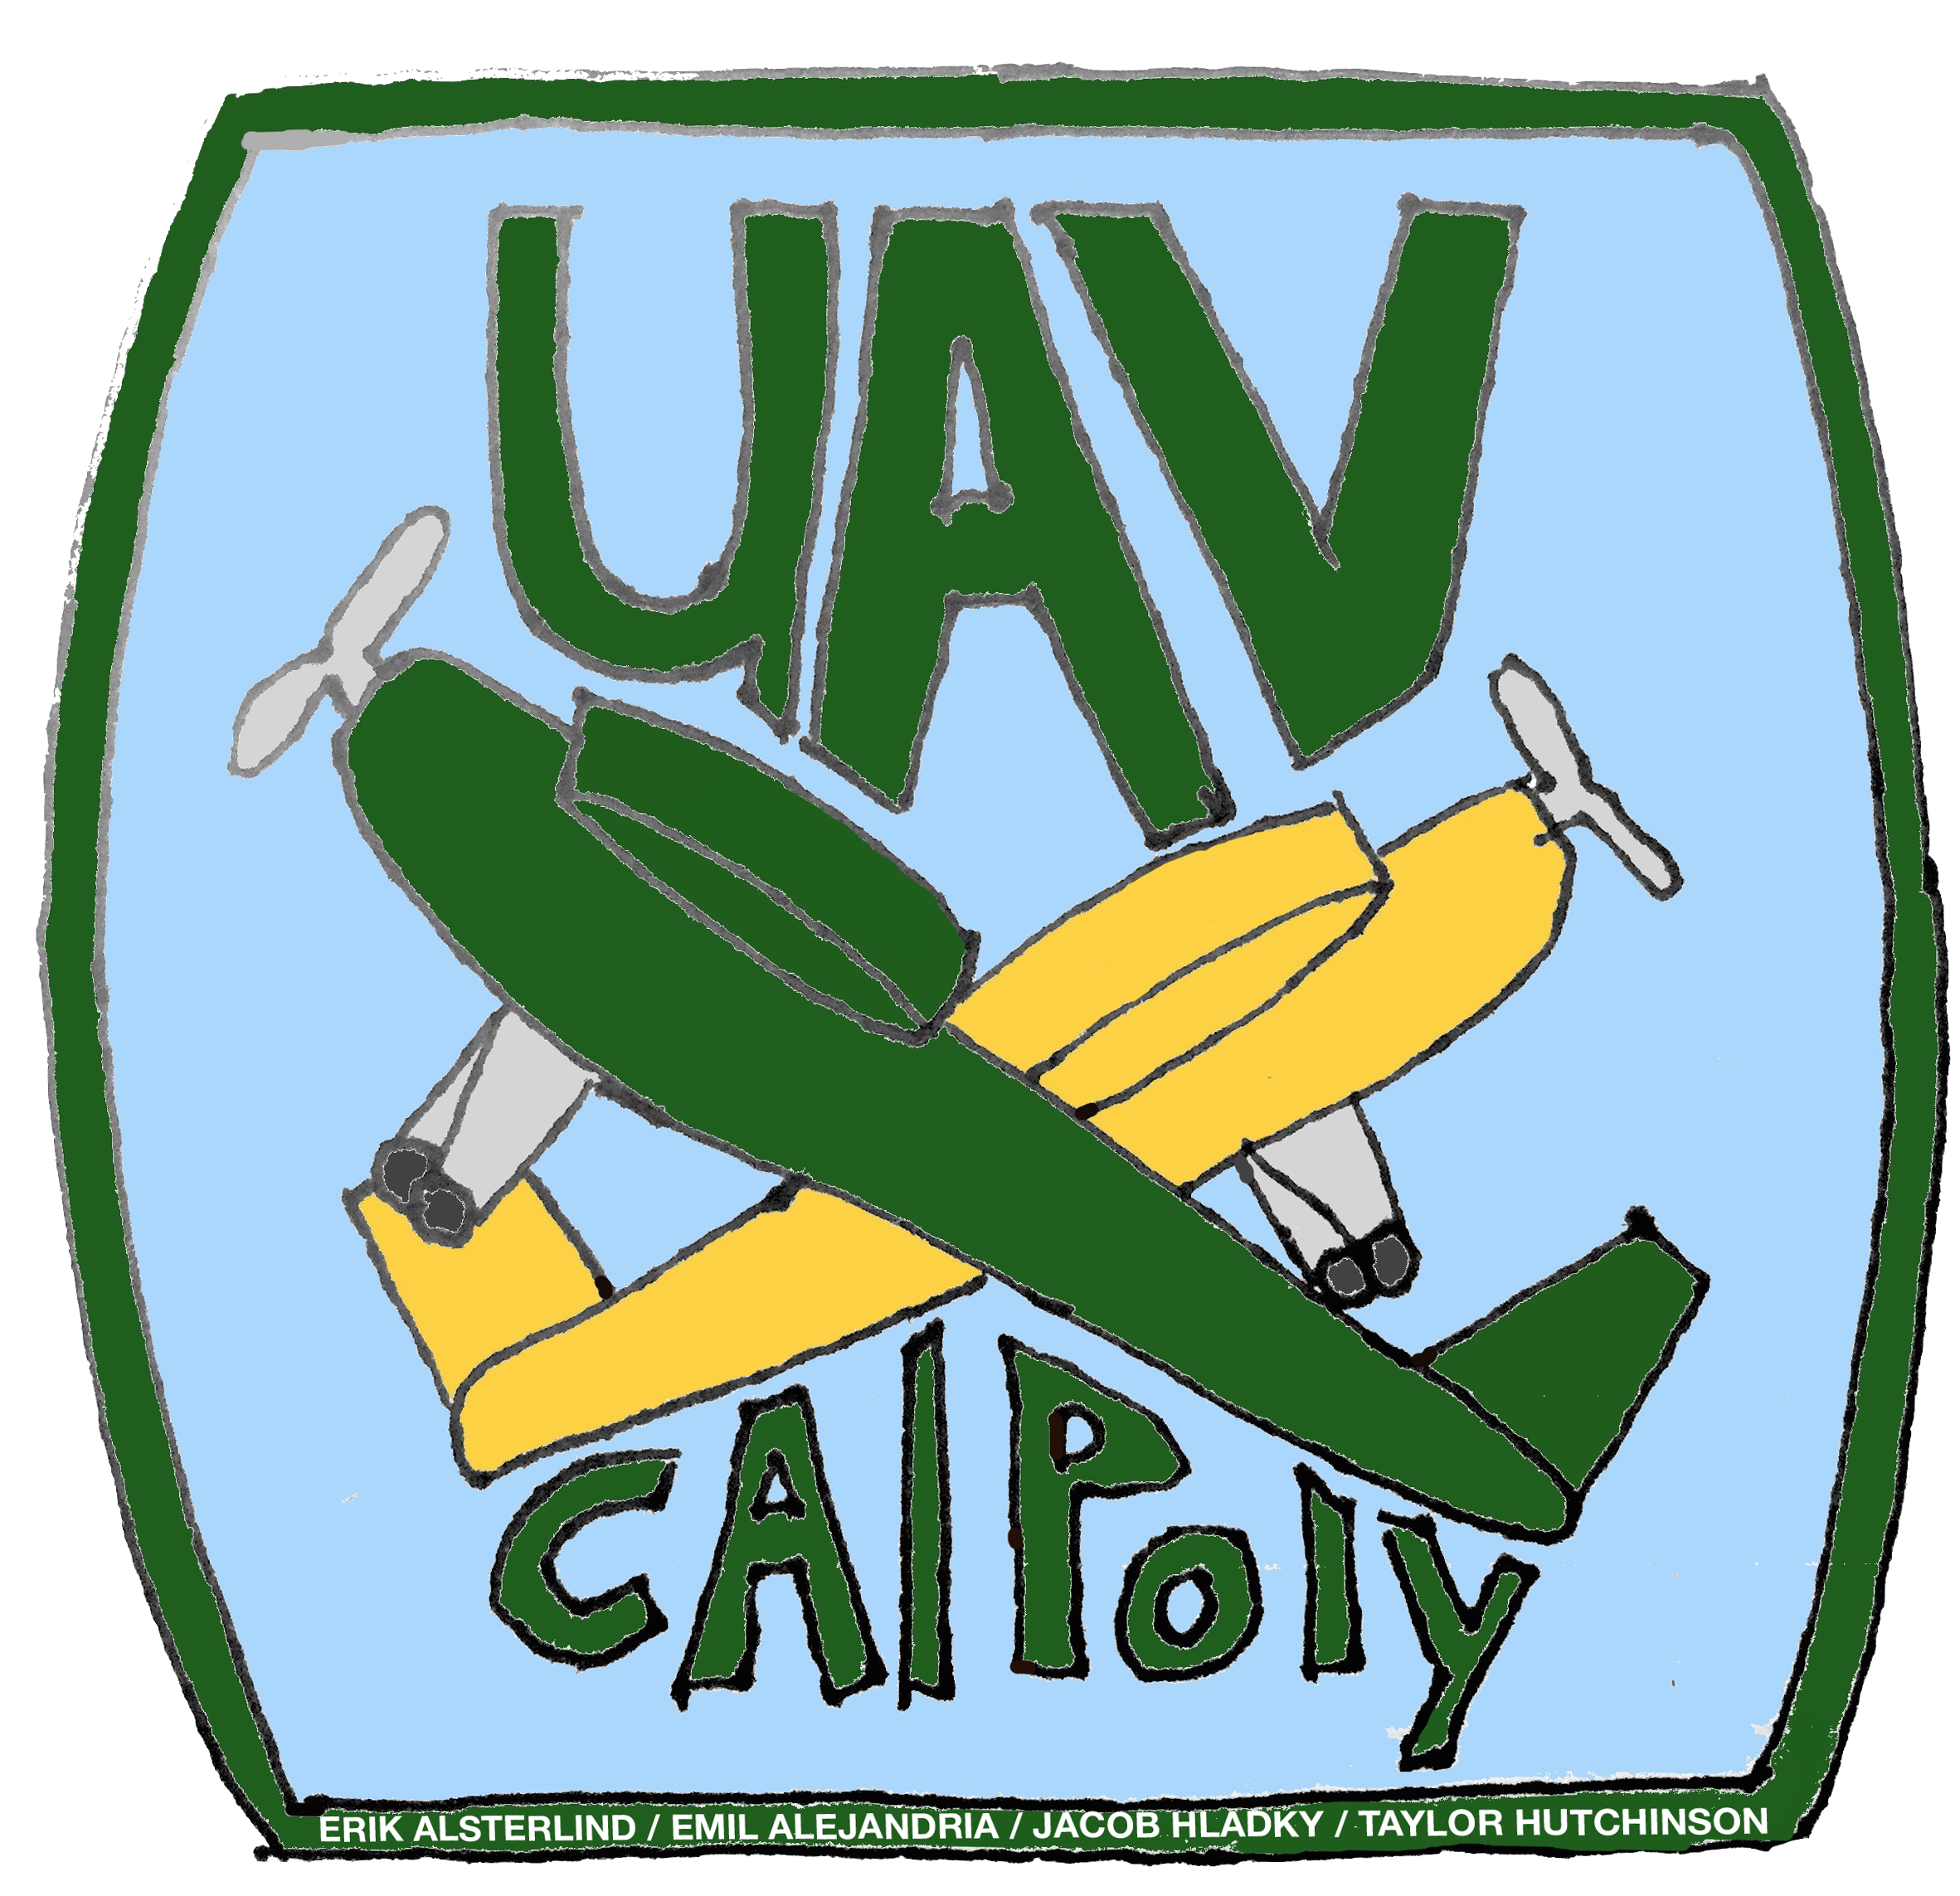
\includegraphics[width=0.5\textwidth]{logo.png}
    \end{figure}

    \vfill {
      \large
      Emil Alejandria\\
      Erik Alsterlind\\
      Jacob Hladky\\
    }

    \vspace{1cm}

    {
      \large
      Department of Computer Engineering\\
      California Polytechnic State University, San Luis Obispo\\
      \today
    }

  \end{center}
\end{titlepage}

\pagenumbering{roman}

\tableofcontents
\clearpage

\pagenumbering{arabic}

\section{Introduction}

\subsection{Project Overview}
The Northrup Grumman UAV project, started three years ago, is a collaborative effort between Cal Poly, San Luis Obispo and Cal Poly, Pomona. This collaboration has resulted in several autonomous vehicles, including several planes, a ground vehicle, and, most recently, a quad-copter. Last year the focus of the project was the implementation of a basic collision avoidance algorithm for the planes. This year, the focus was on maintenance, compatibility, and documentation. Specifically, the goals of this team were to upgrade the autopilot system and to improve the existing collision avoidance algorithm.

The result of this project was a more robust and extensible flight-controller, a more intelligent sense-and-avoid system, and a more accessible code-base.

\subsection{Team Roles}

\begin{itemize}
\item \textbf{Emil Alejandria} --- Team Lead, Sense and Avoid Architect
  \item \textbf{Erik Alsterlind} --- System Architect
  \item \textbf{Jacob Hladky}  --- Development Tools Specialist
\end{itemize}

\subsection{Clients and Community Partners}
Our client on this project is The Northrup-Grumman Corporation (NGC), one of the largest defense companies in the world, and one of the primary contractors for the United States Armed Forces. NGC benefits from continued collaboration with Cal Poly and Cal Poly, Pomona as the universities provide the company a ready supply of talent for potential hire after graduation as well as a possible source for innovation.

Students benefit from NGC's involvement by exposure to the corporate requirements and practices of large, multi-disciplinary projects, and by the opportunity to work on complex hardware systems.

\subsection{Goals and Objectives}
Goals:
\begin{enumerate}
\item Redesign the existing GPS based collision avoidance system to operate more effectively and reliably.
\item Develop a sense and avoidance system for a UAV that is capable of functioning in a GPS denied environment.
\item Design a simulation suite to emulate the real world environment that the planes will be operating in.
\item Emphasize the documentation and organization of the project to aid future capstone teams in improving the project.
\end{enumerate}
Objectives:
\begin{enumerate}
\item Understand the technical capabilities, requirements, and limitations of all potential platforms available to us so that we can select the optimal platform for our needs.
\item Draw a complete picture of environmental variables necessary to design a simulator that can sufficiently emulate a field test.
\item Outline the shortcomings in the project's documentation and work to make documentation a strength of the project rather than a weakness.
\end{enumerate}

\subsection{Results}
Over the course of the year we have implemented a new sense and avoid algorithm that is far more complex and robust than its predecessor. With this algorithm, we have the ability to avoid multiple obstacles and discern an efficient path for reaching our goal safely. The system makes use of GPS information to produce way-points for the auto-pilot to follow. In order to test the algorithm, we feed it sample GPS points that are hard coded into the software to see how it reacts.

We have started the development of a Simulink simulation to try and more accurately model the entire flight system. To run our more sophisticated functionality, we upgraded to a commensurately powerful flight computer. The new hardware is significantly faster than the system it has replaced, and allows us to perform complex calculations with no loss of efficiency. Also, we implemented a communication protocol for sending and receiving GPS information. This protocol was agreed upon with our collaborative partners at Cal Poly, Pomona and provides an effective means of communication between autonomous systems. Finally, throughout this project, we have maintained a standard of stewardship to ensure accessibility for future contributors.

\section{Background}
At the end of the project's previous year, the team was able to successfully demonstrate a functioning sense and avoidance system. The demonstration entailed two autonomous planes, both running the sense and avoid algorithm, flying straight at each other. Once the vehicles got close enough to each other, they both sensed the collision, and altered their paths to turn right and avoid the other plane. Once far enough away from each other, both planes transitioned back to traveling toward their respective targets. While effective, this functionality is limited in its ability to handle different situations. There is little flexibility in what the system can handle, and the path traveled was far from efficient. To eliminate these limitations we have designed our algorithm using two core concepts: potential fields and path projection. By incorporating both we can handle a wide variety of flight situations and minimize the distance traveled while still reaching our goal. Additionally, the greater complexity of our implementation allows for more room to tune and test. As a result, the system can be improved over time.

Similar to the sense and avoid algorithm, last year's hardware setup functioned fine, but was severely limited. The overall processing power of the two micro-controllers was adequate to perform the task at hand, but allowed for little to no expansion. Seeing as we intended to greatly expand the navigation capabilities of the system, we decided to install a superior flight controller to control functionality. A survey of the available autopilot systems resulted in choosing the 3D Robotics Pixhawk because of its POSIX compatibility and prolific processing power. The value of POSIX compliance is its proven value as an industry standard in software applications, which adds credibility and portability to our project.

\section{Engineering Specifications}
\subsection{Specifications}
Discussion of high risk requirements is located in the requirements table below.

\subsubsection{Minimum Avoidance Radius}
This specifies the minimum distance the UAV must be from another UAV or object when it enters collision detection mode. This specification is critical because it corresponds with the turning radius of the UAV and the time the algorithm takes to determine  what to do. If the algorithm detects a collision at a distance less than necessary for avoidance, a collision may occur because there is not enough time or space to avoid the object.

\subsubsection{Collision Recovery Time}
After entering and exiting collision detection mode, several cleanup operations may need to occur. In an airspace that contains another vehicle in flight, the UAV may need to enter collision avoidance mode repeatedly. Thus, the amount of time to reset the collision detection algorithm is critical to operation.

\subsubsection{Fall Back to Manual Control}
If the algorithm malfunctions, it may be necessary to land the UAV to avoid a crash. Thus it is absolutely crucial that the autopilot can be disengaged at any time.

\subsubsection{Collision Priority Delay}
This specification determines which plane has priority over all others during a flight. With the lowest priority, a plane must worry about detection and avoidance at normal specifications. Conversely, a plane with the highest priority does not need to worry about avoidance, and instead stays on a straight path. The purpose of this specification is to create different demonstration situations for testing and validation purposes.

\subsection{Requirements Table}

Risk can be either Low, Medium, or High

\begin{table}[h!]
  \begin{tabulary}{\textwidth}{|C|C|C|C|C|}
    \hline
    \textbf{Spec No.} & \textbf{Parameter Description} & \textbf{Requirement with Units} & \textbf{Tolerance} & \textbf{Risk} \\ \hline
    \multicolumn{5}{|l|}{\textbf{COLLISION DETECTION ALGORITHM REQUIREMENTS}} \\ \hline
    01 & Detection Radius & 500ft & min & H \\ \hline
    02 & Buffer Distance & 50ft & min & M \\ \hline
    03 & Altitude & 70ft & min & L \\ \hline
    04 & Flight Time & 20min & min & L \\ \hline
    05 & Simulation of Collision Detection Algorithm & --- & max & L \\ \hline
    06 & Plane Turning Radius & 20ft & min & M \\ \hline
    07 & Time for Algorithm to Detect Collision & 1s & min & M \\ \hline
    08 & Collision Detection Recovery Time & 5s & 1s & H \\ \hline
    09 & Operating Temperature Range & 50-90 deg F & +/0 5 deg F & L \\ \hline
    10 & Size of Detect Object & 1 sq. ft & max & M \\ \hline
    11 & Time Spent in Collision Avoidance Mode & 1min & 5s & M \\ \hline
    12 & Collision Detect Re-evaluation Interval & .1s & max & H \\ \hline
    13 & Collision Detection in GPS-Limited Area & --- & max & M \\ \hline
    14 & Takeoff/Landing Distance & 300ft & 50ft & L \\ \hline
    15 & Data Logging Interval & .01s & max & M \\ \hline
    16 & Data Communication Interval & 1s & .2s & M \\ \hline
    17 & Collision Detection Control on All Axes & --- & max & M \\ \hline
    18 & Distance for Communication with Partner Plane & 1000ft & 100ft & M \\ \hline
    19 & Distance for Communication with Base Station & 500ft & 50ft & M \\ \hline
    \multicolumn{5}{|l|}{\textbf{SIMULATION ENVIRONMENT REQUIREMENTS}} \\ \hline
    20 & Step Time & 1us & min & M \\ \hline
    21 & Simulation Code Language Support & C++ / C & min & M \\ \hline
    22 & Platform Support & POSIX-Compliant & min & M \\ \hline
    23 & I/O Support & Input and Output Files & min & M \\ \hline
    24 & Error Facility & Report Critical Errors & min & M \\ \hline
    \multicolumn{5}{|l|}{\textbf{CODE STEWARDSHIP REQUIREMENTS}} \\ \hline
    24 & C Code Style & Consistent e.g. K\&R or GNU & min & L \\ \hline
    26 & Code Documentation & Doxygen & min & M \\ \hline
    27 & Warnings & Code Compiled with -Wall, -Wextra, -Werror & min & L \\ \hline
    28 & Licensing & Consistent License for All Code & min & L \\ \hline
  \end{tabulary}
\end{table}

\section{Final Design Overview}
\subsection{The Final Design}
The centerpiece of the hardware setup we installed is the 3D Robotics Pixhawk with PX4 autopilot system. This unit contains a 32-bit ARM processor operating at 168 MHz and running the NuttX Real Time Operating System. This system is replacing the combination of rdupilot Mega and APM 2.6 microcontrollers that were the brains of the previous iteration of this project. The updated hardware system architecture can be seen below in Figure 1.

\begin{figure}[ht!]
   \centering
   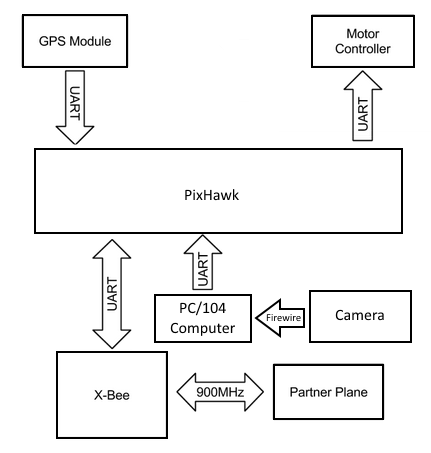
\includegraphics[width=0.5\textwidth]{architecture.png}
   \caption{Final System Architecture}
\end{figure}

The increased word-size of the Pixhawk along with its significantly faster clock rate provides our new system with a much more powerful brain to perform computations and manage modules. We used 3D Robotics GPS modules that came with the Pixhawk to provide GPS points for our sense and avoid algorithm, which plugged into a designated port in the module.

The other hardware component we integrated is the Digi International Xbee S3B Pro radio module for communication between UAVs. The XBee is connected to the Pixhawk via UART serial connection, of which the Pixhawk has three open ports for use. Hardware wise, this connection is relatively simple. The 5 Volt pin of the Pixhawk port goes through a voltage regulator which brings it down to 3.3 Volts for the XBee power pin. The voltage divider is simply comprised of a LM3940 regulator, a 470 nF capacitor across the input, and a 33 uF capacitor across the output. The TX and RX pins of the XBEE and Pixhawk are crossed (TX of Pixhawk port to RX of Xbee and vice versa), and the ground pins are connected.

\begin{figure}[ht!]
  \centering
   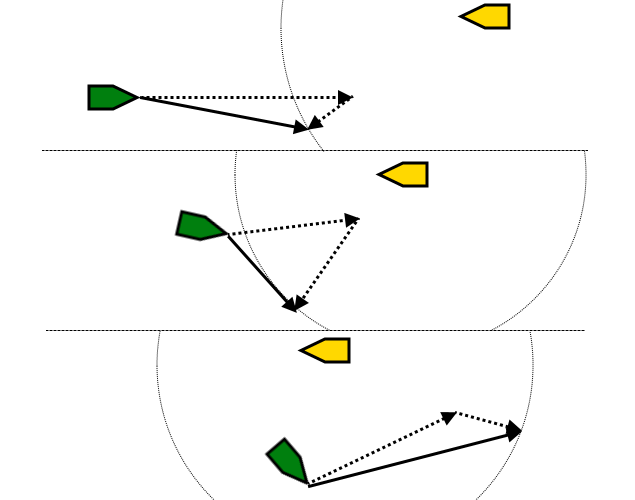
\includegraphics[width=0.5\textwidth]{pushpull.png}
   \caption{The two vectors represent the push away from the other plane and the pull towards the goal}
\end{figure}

In terms of software, the operation of the Xbees is performed through three primary functions. The first function opens and configures the UART Port of the Pixhawk through software. In our code this function is called \textbf{uart\_init()}, and can be reviewed in our software documentation which is listed in the appendix of this report. This function initializes UART settings such as baudrate and flow control. After initialization, we have a function that writes a buffer of data to the XBee, and a function that reads a specific number of bytes of data from the XBee into a buffer. Both functions, \texttt{xbee\_send()} and \texttt{xbee\_recv()}, can be viewed in the aforementioned software documentation.

\begin{figure}[ht!]
   \centering
   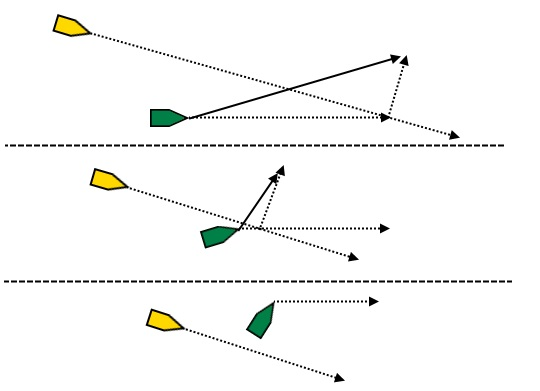
\includegraphics[width=0.5\textwidth]{drift.png}
   \caption{The algorithm sees that it can safely cross the other plane's trajectory and prevent a future collision}
\end{figure}

The design of \texttt{xbee\_recv()} required the accommodation of the real time nature of the system we developed in. Normally, a read() system call in a POSIX environment will return a given size of data as long as it is available to be read. In the Pixhawk, only one byte of data can be read at a time. As a result, we needed to write our function to deal with this difference without losing any data. On top of the main functions we use wrapper functions to provide an additional level of functionality and customization to the software. In Figure 4 below, you can see a software flow diagram of how the uses of the XBee are integrated into the software of the system using our functions.

\begin{figure}[ht!]
   \centering
   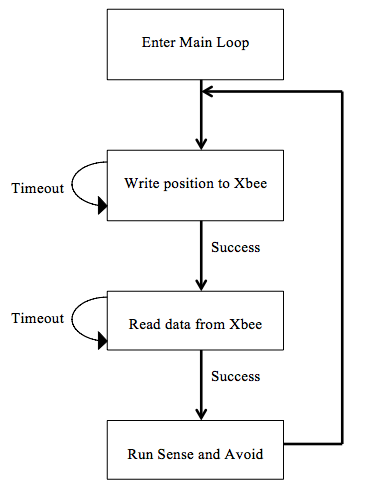
\includegraphics[width=0.5\textwidth]{flow.png}
   \caption{The software flow architecture of our program}
\end{figure}

Part of our collaboration with the Cal Poly, Pomona team was a common system of communication between autonomous vehicles. The standard that we agreed upon resulted in two types of packets that can be sent on the network. The structure of the bodies of the packets can be seen below in Figures 5 and 6. One is a system status packet that the Pomona team uses in its Ground Station to map the functionality of planes during a demonstration.

The other is a global position packet that contains GPS data that the planes need to communicate with each other for collision avoidance to function properly. The bodies of these packets contain different information, but both utilize the same general header structure. This header contains values that define what packet is being sent as well as a sync word and a checksum value to validate a packet upon its arrival. Complete documentation of the packet structure can be found in the source code.

\begin{centering}
\begin{Verbatim}[fontsize=\scriptsize]
	typedef struct {
	   int32_t sync;
	   uint8_t source_id;
	   uint8_t dest_id;
	   uint8_t seq;
	   uint8_t ttl;
	   uint16_t message_type;
	   uint16_t message_length;
	   int8_t checksum;
	} header_t __attribute__((packed));
\end{Verbatim}
Figure 5: Structure of status packet body

\begin{Verbatim}[fontsize=\scriptsize]
	typedef struct {
	   int64_t time_stamp;
	   uint16_t vehicle_id;
	   uint8_t vehicle_mode;
	   uint8_t vehicle_state;
	} status_body_t __attribute__((packed));
\end{Verbatim}
Figure 6: Structure of position packet body\par
\end{centering}
\bigskip

The sense and avoidance system utilizes two algorithms to determine how best to avoid any potential collisions. The algorithms each generate a pair of north and east vectors which are summed to produce a vector pointing in the optimal direction for preventing collisions. The first algorithm, called the potential field method, pushes the plane directly away from obstacles and pulls the plane toward the objective. The magnitude of the pull is constant, but the magnitude of the push varies which helps to improve pathing efficiency. The second algorithm attempts to predict and avoid future collisions. It calculates whether the plane's trajectories intersect and, if they do, the time until any collisions. It then attempts to decide whether the safest and most efficient course of action would be to proceed normally, speed up, or deviate slightly from the current flight path. The first algorithm doesn't take into consideration future situations and the second algorithm neglects more immediate hazards. By combining these two algorithms we can utilize the strengths of both as a work around to each other's weakness.

\subsection{Safety Concerns}
The primary concern with the system is for the safety of the planes in flight, and for any bystanders that might view future demonstrations. To ensure that no damage is done we have developed methods of simulating our sense and avoid algorithm before putting anything in the air. The first aspect of simulation involves hard coding sample data points into the software being run on the Pixhawk. By providing a variety of different sample GPS data, we can comprehensibly test how the algorithm responds to different situations, and tune our system as necessary. The second aspect is a Simulink simulation developed to model the entire system and see how it responds as realistically as possible. Having a simulation outside the Pixhawk environment allows us to make relatively major changes and test them without having to touch the actual functioning software. With these tools, we can make sure our system is prepared for physical testing without having to take major risks with costly hardware or anyone's wellbeing.

\subsection{Project Cost}

\section{System Integration and Testing}
\subsection{FMEA}
Our FMEA Identified 3 major points of failure, each with a few specific ways it could fail. Those points of failure are:
\begin{enumerate}
\item UAV Platform - the hardware keeping the UAV in the air fails in some way. Methods of failure:
  \begin{itemize}
  \item Loss of control
  \item Engine failure
  \item Loss of power
  \end{itemize}
These failures are addressed by the platform team within the UAV group.
\item Pixhawk Failure - software or hardware problems related to the Pixhawk. Methods of failure:
  \begin{itemize}
  \item Algorithm failure
  \item Hardware failure
  \end{itemize}
  Algorithm failure means that we located an obstacle, but failed to avoid it. Hardware failure, on the other hand, would be electric failure of the Pixhawk and its peripherals.
\item XBee Failure - the communication is interrupted or invalidated somehow. Methods of failure:
  \begin{itemize}
  \item Loss of connection
  \item Bad data
  \end{itemize}
\end{enumerate}
These and other possible failures are all addressed in our risk management document included with this report.

\subsection{DVP+R}
The following tests were explored in our DVP+R:
\begin{itemize}
\item \textbf{Pixhawk Resilience Test:} subjecting the Pixhawk to physical stress similar to what it would endure while in flight to ensure integrity.
\item \textbf{Object Detection Test:} place multiple objects / planes in the environment and ensure that the system identifies all of them.
\item \textbf{Beacon Test:} Place GPS beacons in the flight area and ensure that the system avoids them.
\item \textbf{Waypoint Test:} Have plane navigate through an environment with obstacles and ensure it arrives within 10m of waypoint.
\item \textbf{Connection Verification Test:} Send packets via XBee in potentially restricted environments (different planes, different orientations, etc) and ensure data arrives.
\item \textbf{Packet Verification Test:} Send packets via XBee in potentially restricted environments and ensure data validity.
\item \textbf{IMU Test:} Move the hardware while the IMU is running to test for accuracy
\end{itemize}

Other tests explored applied to the platform team but not to this team. They can be found in the DVP+R Section of the appendix.

\subsection{Overall System Analysis}
\subsubsection{Collision Avoidance Algorithm}
Current tests indicate that our algorithm is able to make limited predictions to prevent collisions and is able to maintain a minimum distance from any obstacles while taking an efficient path. The performance of the algorithm meets and exceeds expectations, giving us the potential to continually build upon the algorithm without concern of straining system resources. More testing is necessary as our test suite is currently limited to emulated algorithm behavior.

\subsubsection{Simulation Environment}
The simulation suite currently consists of emulating the algorithm behavior in software and modeling a realistic system in Simulink. The algorithm emulation is sufficient for determining basic functionality and making tweaks to the algorithm. The system modeling is done in Simulink where parameters are used to more closely replicate the plane's movements as well as environmental factors.

\subsubsection{Code Stewardship}
We have adhered to an established standard of documentation for everything we develop in order to to enhance accessibility for future contributors as well as anyone curious about the project.  We have also placed all our code on a github repository for easy access and management. The private repo is provided to us by the IEEE club and is called the “Cal Poly IEEE/firmware” repository.

\subsubsection{Future Plans}
The sense-and-avoid algorithm is depends on consistent, accurate GPS data. A line-fitting algorithm should be implemented to improve trajectory projection. This will also prevent failure in the case of communication loss by predicting and adjusting the plane's path. A Kalman filter should be implemented on the GPS data to improve both the current accuracy of calculations and the accuracy of any future path prediction algorithms.

The software simulation for the algorithm needs minor improvements, however emphasis will be placed on developing the simulator in Simulink. While the framework is in place to model the system, the algorithm needs to be correctly ported into Simulink in order for testing to be completely useful.

More thorough testing needs to be performed on the autopilot software. This year we were not permitted to fly so we were unable to perform any practical testing. We have reviewed the autopilot documentation and have a fairly good idea of how it will function within our environment, but that understanding needs to be implemented and tested before any major demonstration can be performed. The autopilot functionality of the previous year's system could be used as a reference.

The voltage regulator for the XBee radios should be implemented on a PCB or proto-board. The current circuit is prototyped on a breadboard and may not withstand the rigors of flight.

\section{Appendices}
PDFs for the FMEA, DVP+R, Decision Matrix, Processes for Handling Risks, and Personas will be included with this report.

\end{document}
